\section{Analysis of Results}

\subsection{Morris Method Global Analysis Results}
A global sensitivity analysis using the Morris method was performed to identify the most influential parameters on the total profit metric for both the DDPG and SAC agents. This analysis is crucial for understanding which factors drive agent performance and for revealing differences in their learned policies.

\begin{figure}[H]
    \centering
    \begin{subfigure}{0.49\textwidth}
        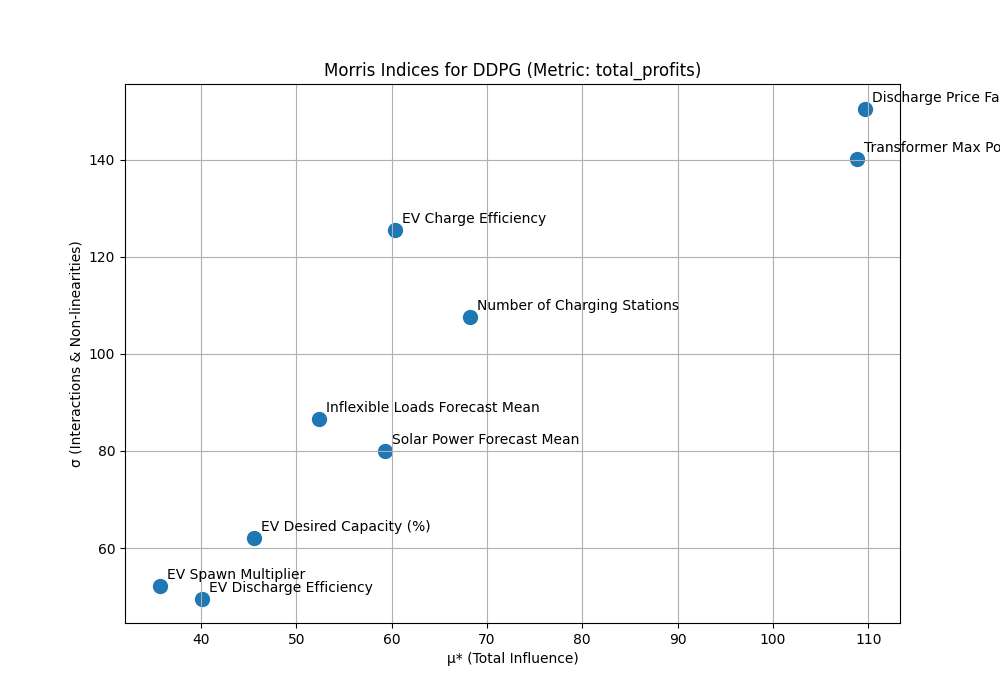
\includegraphics[width=\linewidth]{../sensitivity_analysis_results/Morris_20251021_091828/morris_plot_DDPG.png}
        \caption{Morris Analysis for DDPG}
        \label{fig:morris_ddpg}
    \end{subfigure}
    \hfill
    \begin{subfigure}{0.49\textwidth}
        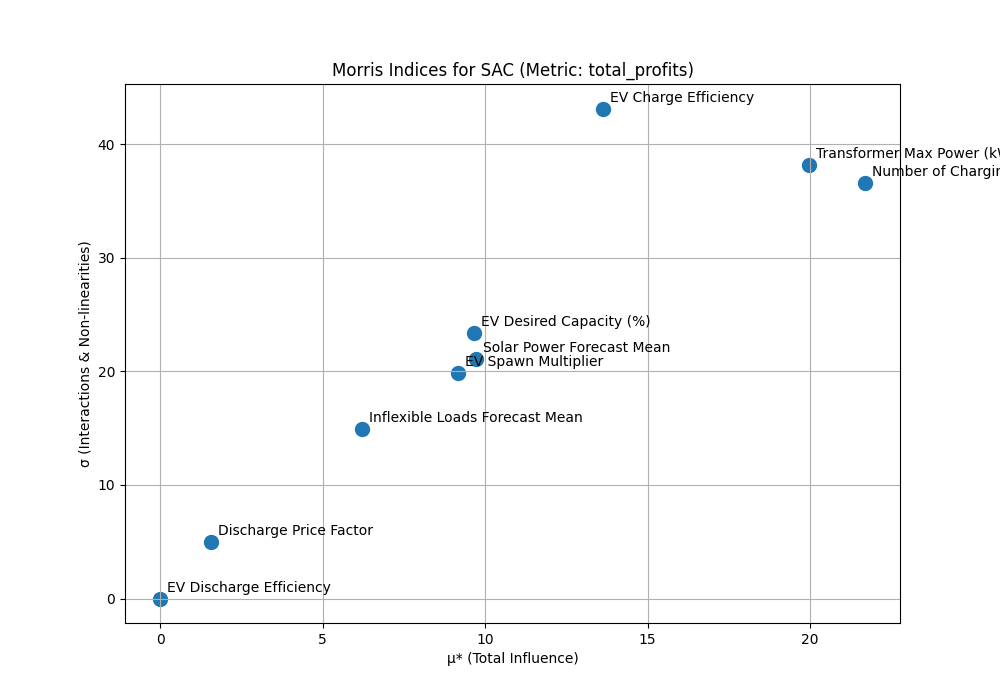
\includegraphics[width=\linewidth]{../sensitivity_analysis_results/Morris_20251021_211648/morris_plot_SAC.png}
        \caption{Morris Analysis for SAC}
        \label{fig:morris_sac}
    \end{subfigure}
    \caption{Morris sensitivity analysis plots for DDPG and SAC. The comparison reveals both shared sensitivities and critical differences in their learned strategies.}
    \label{fig:morris_plots_comparison}
\end{figure}

\subsubsection{Critical Interpretation and Comparison}

A detailed examination of the plots in Figure \ref{fig:morris_plots_comparison} reveals key differences in what each agent learned to prioritize.

\begin{itemize}
    \item \textbf{Shared Dominant Factor:} For both DDPG and SAC, the \textbf{Transformer Max Power} stands out with a very high mean effect ($\mu^*$) and a high standard deviation ($\sigma$). This is an expected and reassuring result, confirming that both agents correctly identified the Trasformer Power as a key element to consider.

    \item \textbf{Divergence in Secondary Factors:} The most interesting insights come from the secondary parameters. For the \textbf{DDPG} agent, the \textbf{Discarge price factor} is the next most influential parameters. This suggests that DDPG's deterministic policy is highly focused on price spread.

    \item In stark contrast, the \textbf{SAC} agent displays a high sensitivity to \textbf{EV Charge Efficiency} , \textbf{Number of Charging Stations} and Maximum Transformer Power (this last one is enforced by the OAT analysis see \ref{fig:oat_transformer_degradation_sac}) all of these have high $\mu^*$ and $\sigma$. The sensitivity to charge efficiency is particularly noteworthy and was not observed in the DDPG agent. This suggests that SAC's stochastic and more exploratory policy learns to exploit the subtle, non-linear effects of charging efficiency, perhaps by identifying specific conditions where small efficiency gains lead to disproportionately large profit increases.
\end{itemize}

\subsection{One-at-a-Time (OaaT) Results}
The OaaT analysis further clarifies the direct relationships between key parameters and system outputs.



\begin{figure}[H]
    \centering
    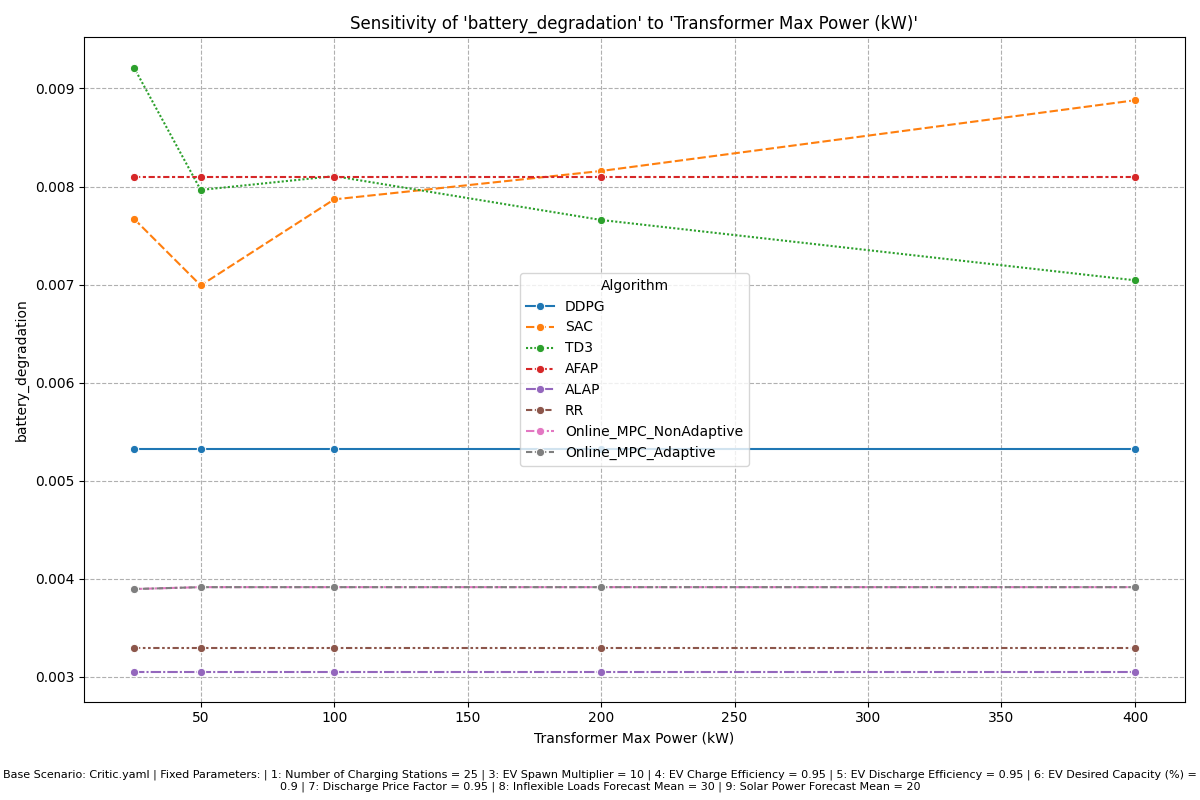
\includegraphics[width=0.8\linewidth]{../sensitivity_analysis_results/Risultati_scelti/sensitivity_Transformer_Max_Power_(kW)_vs_battery_degradation.png}
    \caption{Impact of maximum transformer power on battery degradation for the SAC algorithm.}
    \label{fig:oat_transformer_degradation_sac}
\end{figure}
\noindent
Figure \ref{fig:oat_transformer_degradation_sac} provides further confirmation of the significant influence of \textbf{Maximum Transformer Power} on battery degradation for the SAC agent, as identified by Morris' analysis.  This highlights how adequate transformer sizing is crucial to mitigate battery degradation and optimize the useful life of SAC-managed EVs.





\begin{figure}[H]
    \centering
    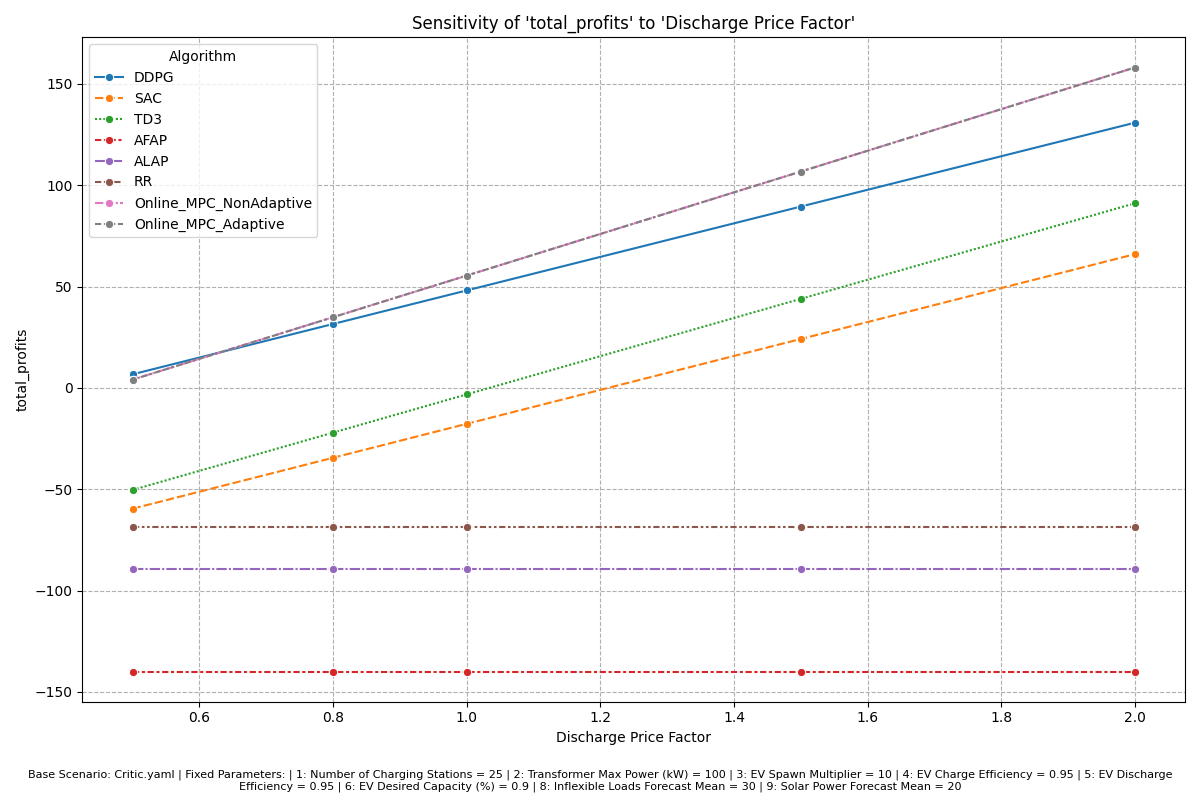
\includegraphics[width=0.8\linewidth]{../sensitivity_analysis_results/Risultati_scelti/sensitivity_Discharge_Price_Factor_vs_total_profits.png}
    \caption{Impact of Discharge Price Factor on Total Profits for various algorithms.}
    \label{fig:oat_discharge_profit}
\end{figure}

As shown in Figure \ref{fig:oat_discharge_profit}, for all V2G-capable algorithms (SAC, DDPG, MPC), profit increases substantially as the \textbf{Discharge Price Factor} rises above 1.0. This confirms the finding from the Morris analysis that this is the most critical economic lever. Heuristic algorithms that do not discharge (AFAP, ALAP) are, as expected, unaffected.

\begin{figure}[H]
    \centering
    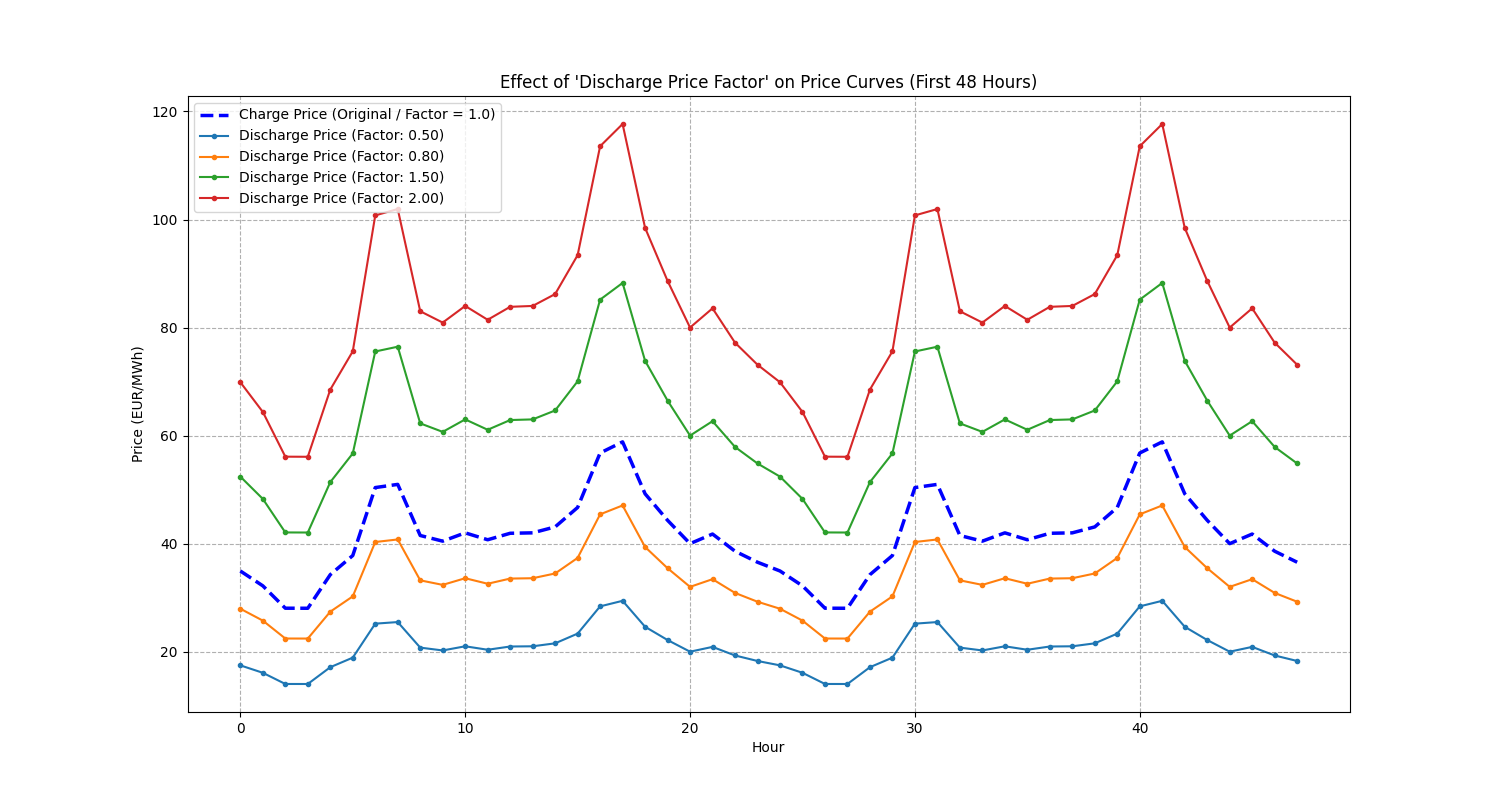
\includegraphics[width=0.8\linewidth]{../sensitivity_analysis_results/Risultati_scelti/price_curves_vs_discharge_factor.png}
    \caption{Illustration of how the discharge price (selling price) changes relative to the charge price (buying price) based on the discharge price factor.}
\end{figure}
\noindent
Figure \ref{fig:price_curves} provides a visual explanation for the results in the previous plot, showing how a factor greater than 1.0 makes the selling price consistently higher than the buying price, creating clear arbitrage opportunities.

\begin{figure}[H]
    \centering
    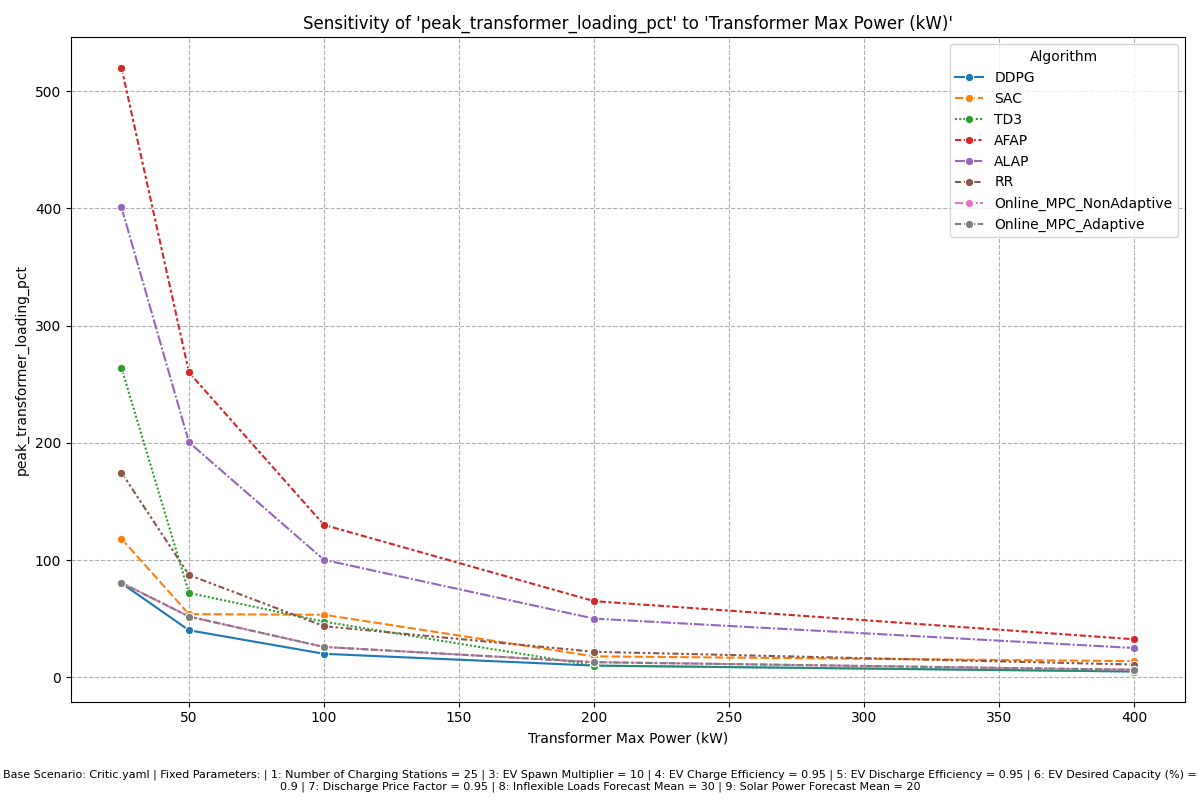
\includegraphics[width=0.8\linewidth]{../sensitivity_analysis_results/Risultati_scelti/sensitivity_Transformer_Max_Power_(kW)_vs_peak_transformer_loading_pct.png}
    \caption{Impact of Transformer Max Power on Peak Transformer Loading.}
    \label{fig:oat_transformer_load}
\end{figure}
\noindent
Figure \ref{fig:oat_transformer_load} illustrates the direct impact of transformer capacity on grid stress. For unintelligent algorithms like AFAP, peak loading remains dangerously high until the transformer capacity is significantly oversized. In contrast, proactive controllers like DDPG, and MPC adapt their behavior to respect the transformer's limit, keeping peak load consistently below 100\% across a wide range of capacities. This demonstrates their crucial role in maintaining grid stability.However TD3 shows that without proper optimization cannot go well then DDPG even though it's a DDPG improvement.

\begin{figure}[H]
    \centering
    \includegraphics[width=0.8\linewidth]{\detokenize{../sensitivity_analysis_results/Risultati_scelti/sensitivity_EV_Desired_Capacity_(\%)_vs_average_user_satisfaction.png}}
    \caption{Impact of EV Desired Capacity on Average User Satisfaction.}
    \label{fig:oat_desired_capacity}
\end{figure}
\\
\noindent
Figure \ref{fig:oat_desired_capacity} shows that as the users' desired state of charge increases, it becomes more challenging for all algorithms to achieve high satisfaction. Notably, heuristic algorithms like AFAP and ALAP maintain near-perfect satisfaction as they have a singular focus on charging, whereas the more intelligent agents must balance this goal against others like profit maximization and grid stability.

\subsection{Reward Function and Curriculum Learning Analysis}
A key contribution of this work was the development of the \textbf{FastProfitAdaptiveReward} function and a Curriculum Learning (CL) strategy to improve agent training.

\begin{figure}[H]
    \centering
    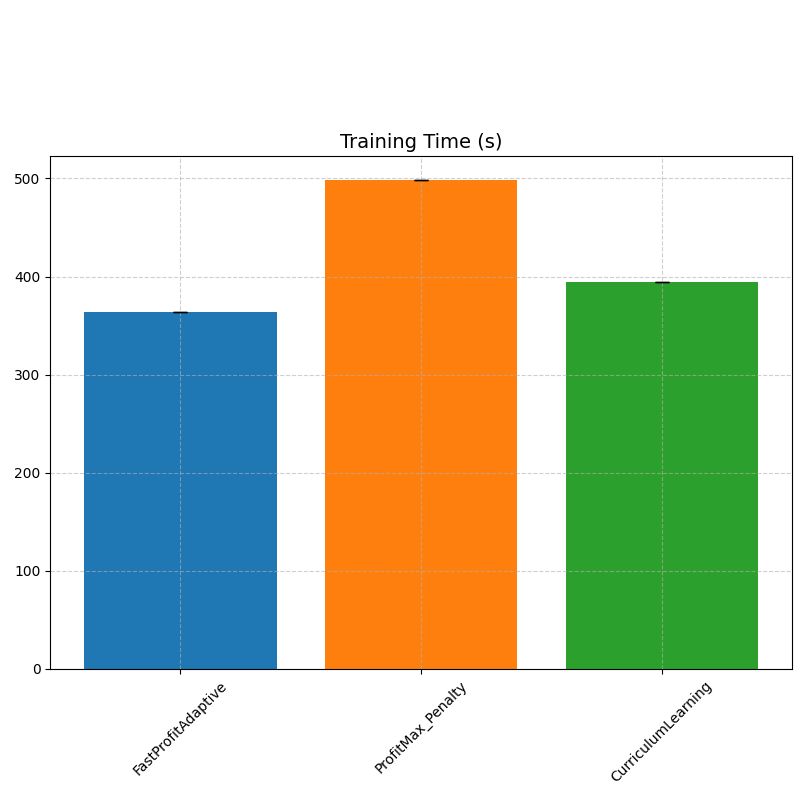
\includegraphics[width=0.5\textwidth]{../sensitivity_analysis_results/Risultati_scelti/performance_summary_RewardFunctionComparison.png}
    \caption{Training time performance comparison between the original reward function (\textbf{ProfitMax\_Penalty}) and the new adaptive function (\textbf{FastProfitAdaptive}), with and without Curriculum Learning.}
    \label{fig:reward_comparison_summary}
\end{figure}

\begin{figure}[H]
    \centering
    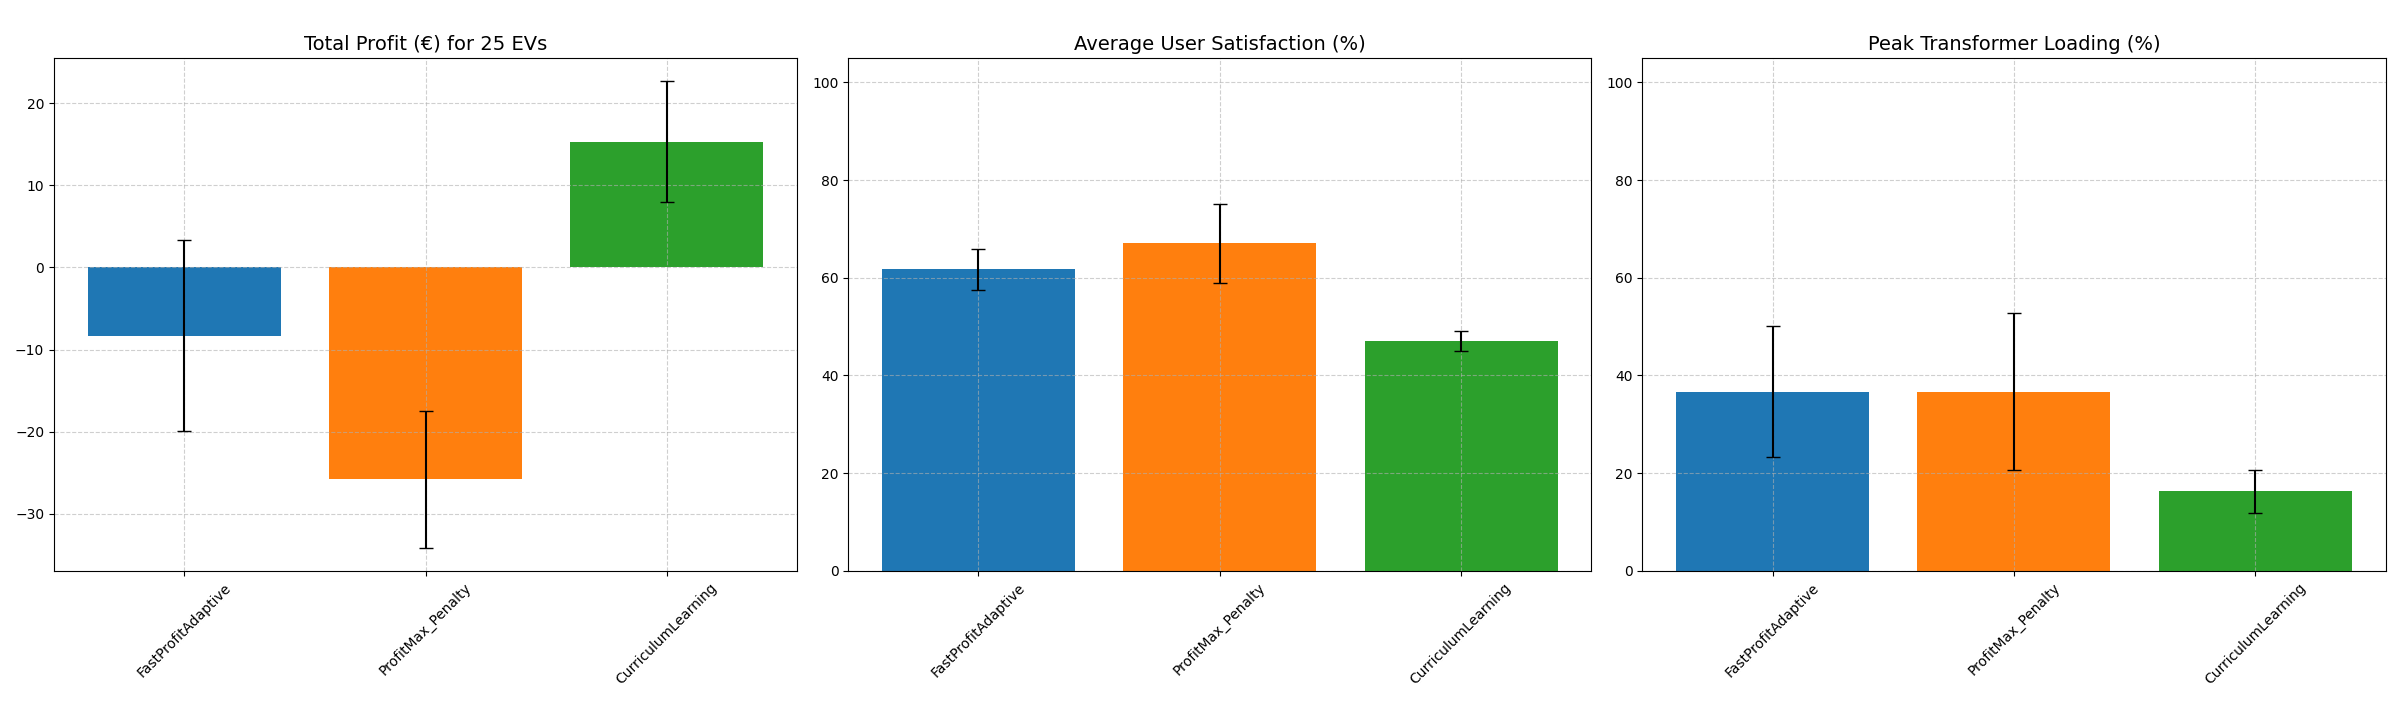
\includegraphics[width=0.7\textwidth]{../sensitivity_analysis_results/Risultati_scelti/RewardFunctionComparison_profit.png}
    \caption{Performance comparison on the KPI between the original reward function (\textbf{ProfitMax\_Penalty}) and the new adaptive function (\textbf{FastProfitAdaptive}), with and without Curriculum Learning.}
    \label{fig:reward_comparison_summary_2}
\end{figure}
\noindent
As summarized in Figure \ref{fig:reward_comparison_summary_2}, the DDPG agent trained with the CL method significantly outperforms the one trained with the original, achieving higher profits and better overall performance because it uses both the advantage of the two reward funtions.
\begin{figure}[H]
    \centering
    \begin{subfigure}{0.49\textwidth}
        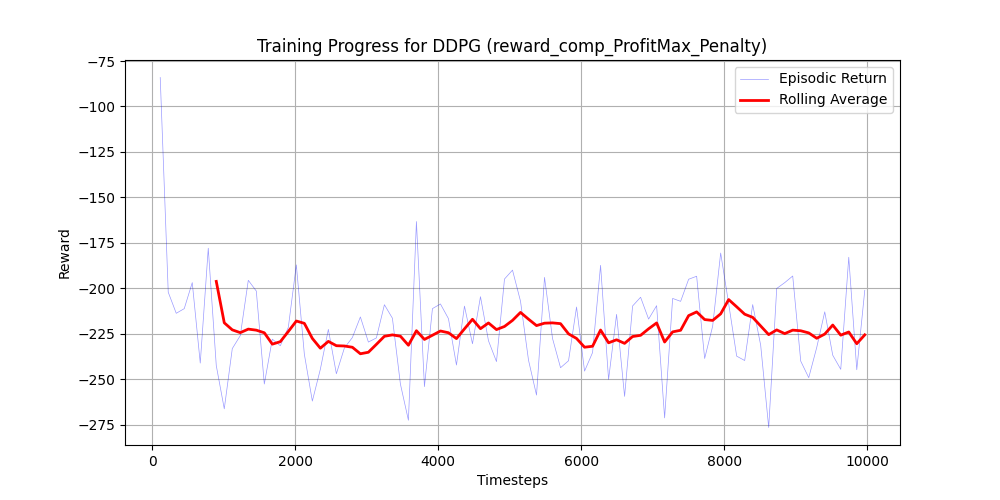
\includegraphics[width=\linewidth]{../sensitivity_analysis_results/Risultati_scelti/DDPG_reward_comp_ProfitMax_Penalty_20251022_084014.png}
        \caption{Original Reward}
    \end{subfigure}
    \hfill
    \begin{subfigure}{0.49\textwidth}
        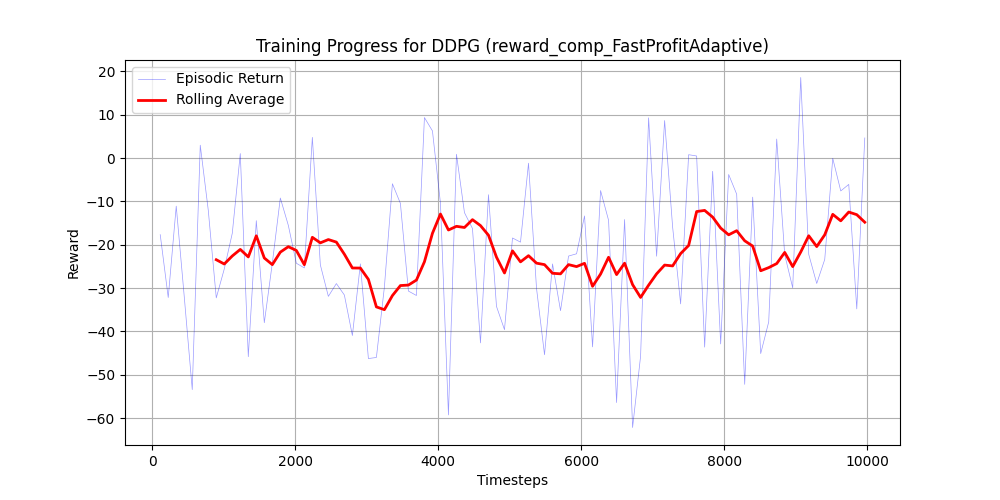
\includegraphics[width=\linewidth]{../sensitivity_analysis_results/Risultati_scelti/DDPG_reward_comp_FastProfitAdaptive_20251022_083514.png}
        \caption{New Adaptive Reward}
    \end{subfigure}
    \caption{Comparison of training progress for DDPG with the original vs. the new adaptive reward function. The new function leads to a more stable and consistently positive reward signal during training.}
    \label{fig:ddpg_rewards}
\end{figure}

\subsubsection{Curriculum Learning Stages}
The CL strategy involved two stages:
\begin{enumerate}
    \item \textbf{Stage 1 (First 5000 steps):} The agent is trained with the original \textbf{ProfitMax\_Penalty} reward, forcing it to first learn basic constraint satisfaction.
    \item \textbf{Stage 2 (After 5000 steps):} The reward function switches to the new \textbf{FastProfitAdaptiveReward}, encouraging the agent to build upon its foundation of safe behavior to explore more profitable strategies.
\end{enumerate}

\begin{figure}[H]
    \centering
    \begin{subfigure}{0.49\textwidth}
        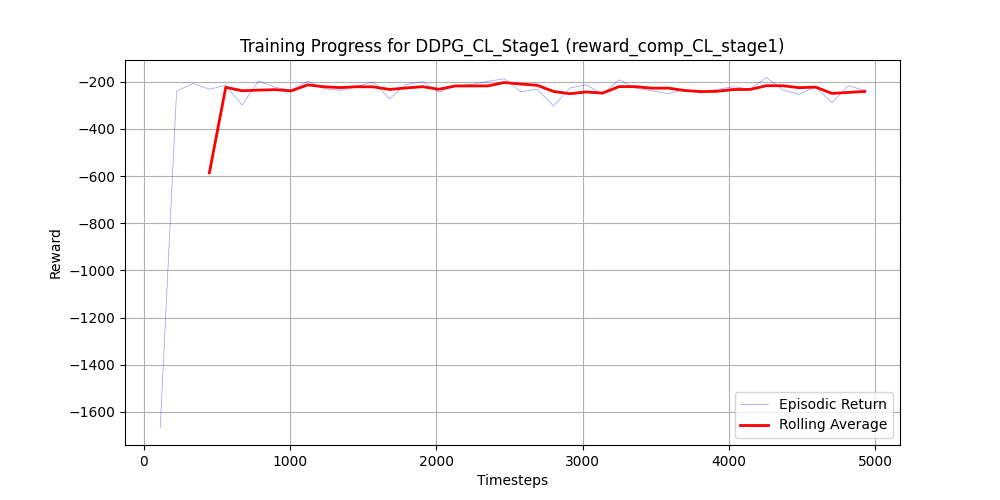
\includegraphics[width=\linewidth]{../sensitivity_analysis_results/Risultati_scelti/DDPG_CL_Stage1_reward_comp_CL_stage1_20251022_084237.png}
        \caption{CL Stage 1: Learning basic constraints.}
    \end{subfigure}
    \hfill
    \begin{subfigure}{0.49\textwidth}
        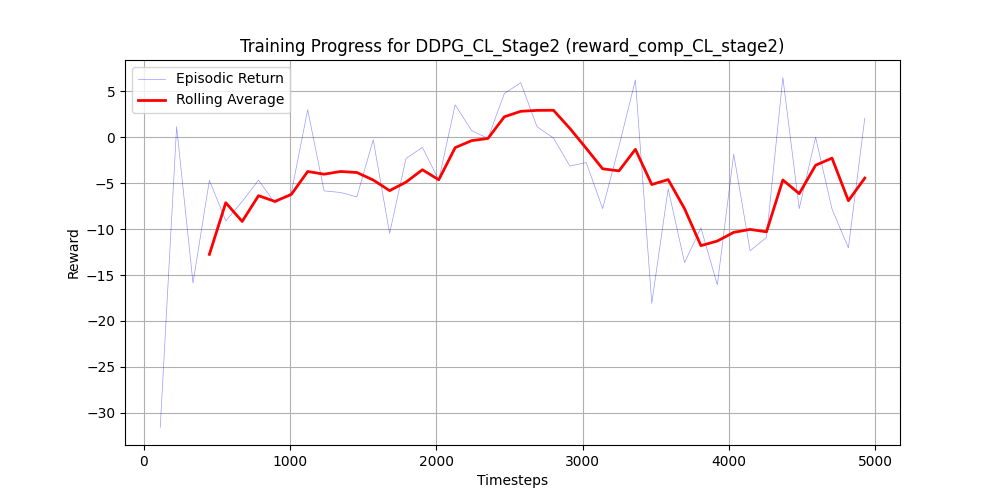
\includegraphics[width=\linewidth]{../sensitivity_analysis_results/Risultati_scelti/DDPG_CL_Stage2_reward_comp_CL_stage2_20251022_084506.png}
        \caption{CL Stage 2: Optimizing for profit.}
    \end{subfigure}
    \caption{Training progress during the two stages of Curriculum Learning. A clear and significant improvement in reward is visible upon switching to the adaptive reward function in Stage 2, demonstrating the effectiveness of the CL strategy.}
    \label{fig:cl_stages}
\end{figure}

Figure \ref{fig:cl_stages} clearly shows the success of this approach. In Stage 2, the agent's reward immediately and consistently climbs to a much higher level than what was achievable with either reward function alone. This confirms that by first establishing a baseline of safe behavior and then optimizing for profit, the CL strategy enables the agent to discover superior policies.
